\section{The \pktlanguage compiler}

% TODO: The compiler's biggest contribution is separating out the stateful
% portions of the architecture from the stateless ones.

% And this is important, because the stateless ones can ALWAYS be implemented,
% while the stateful ones are more constrained.

% Like Hari said, the critical path scheduling doesn't affect feasibility.
% It only affects optimality.

% The hardest thing about the compiler is the stateful vs. stateless separation.
% And mapping the stateful operations to the hardware constraints.

% But at the same time, not having the pipeline/crit. path scheduling makes it
% a tool, not a compiler anymore.

\label{s:compiler}

\begin{figure*}[!t]
  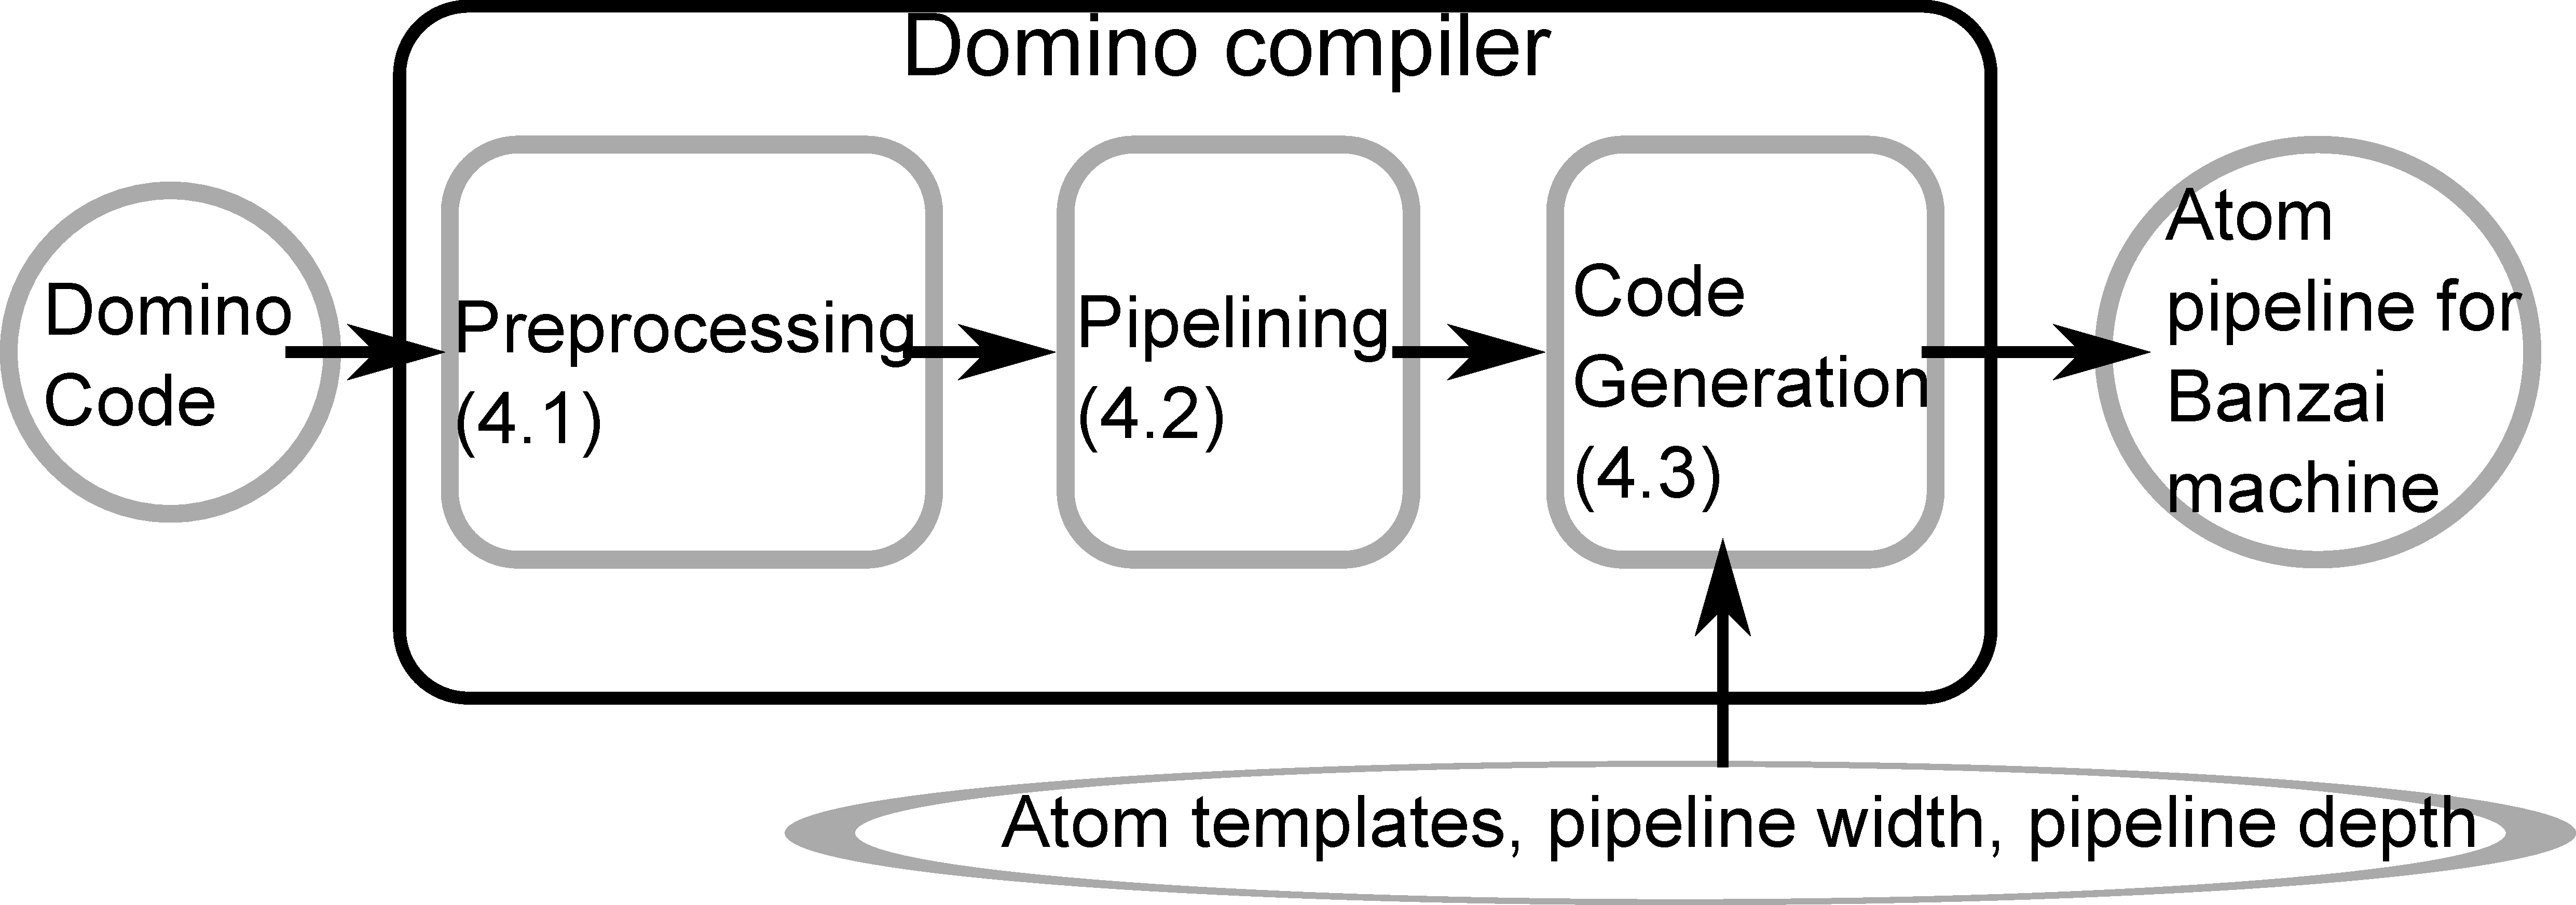
\includegraphics[width=\textwidth]{compiler.pdf}
  \caption{Passes in the \pktlanguage compiler}
  \label{fig:passes}
\end{figure*}

\begin{figure*}[!t]
  \hspace{-0.3in}
  \begin{minipage}{0.55\textwidth}
  \begin{small}
  \begin{lstlisting}[style=customc, numbers=none, frame=none]
  if (@\textcolor{blue}{pkt.arrival - last\_time[pkt.id] > THRESHOLD}@) {
    saved_hop[pkt.id] = pkt.new_hop;
  }
  \end{lstlisting}
  \end{small}
  \end{minipage}
%  
  \hspace{-0.5in}
  $\Longrightarrow$ 
  \hspace{-0.3in}
%  
  \begin{minipage}{0.6\textwidth}
  \begin{small}
  \begin{lstlisting}[style=customc, numbers=none, frame=none]
  @\textcolor{blue}{pkt.tmp = pkt.arrival - last\_time[pkt.id]  > THRESHOLD}@;
  saved_hop[pkt.id] = @\textcolor{magenta}{// Rewritten}@
    @\textcolor{blue}{pkt.tmp}@ ? pkt.new_hop : saved_hop[pkt.id];
  \end{lstlisting}
  \end{small}
  \end{minipage}
\vspace{-.2in}
\caption{Conversion to straight-line code}
\label{fig:if_convert}
\end{figure*}

\begin{figure*}[!t]
  \begin{minipage}{0.43\textwidth}
  \begin{small}
  \begin{lstlisting}[style=customc, numbers=none, frame=none]
pkt.id = hash2(pkt.sport,
               pkt.dport)
         % NUM_FLOWLETS;
...
@\textcolor{blue}{last\_time[pkt.id] = pkt.arrival;}@
...
  \end{lstlisting}
  \end{small}
  \end{minipage}
%  
  \hspace{-0.5in}
  $\Longrightarrow$ 
  \hspace{-0.2in}
%  
  \begin{minipage}{0.61\textwidth}
  \begin{small}
  \begin{lstlisting}[style=customc, numbers=none, frame=none]
pkt.id = hash2(pkt.sport,           @\textcolor{magenta}{// Read flank}@
               pkt.dport)
         % NUM_FLOWLETS;
pkt.last_time = last_time[pkt.id];  @\textcolor{magenta}{// Read flank}@
...
@\textcolor{blue}{pkt.last\_time = pkt.arrival;}@             @\textcolor{magenta}{// Rewritten}@
...
last_time[pkt.id] = pkt.last_time;  @\textcolor{magenta}{// Write flank}
  \end{lstlisting}
  \end{small}
  \end{minipage}
  \caption{Adding read and write flanks}
\label{fig:stateful_flanks}
\end{figure*}

\begin{figure*}[!t]
  \begin{minipage}{\textwidth}
  \begin{minipage}{0.4\textwidth}
  \begin{small}
  \begin{lstlisting}[style=customc, numbers=none, frame=none]
@\textcolor{blue}{pkt.id}@ = hash2(pkt.sport,
              pkt.dport)
              % NUM_FLOWLETS;
@\textcolor{blue}{pkt.last\_time}@ = last_time[@\textcolor{blue}{pkt.id}@];
...
@\textcolor{blue}{pkt.last\_time}@ = pkt.arrival;
last_time[@\textcolor{blue}{pkt.id}@] = @\textcolor{blue}{pkt.last\_time}@;
  \end{lstlisting}
  \end{small}
  \end{minipage}
 % 
  %\hspace{-0.1in}
  $\Longrightarrow$
  \hspace{-0.2in}
%
  \begin{minipage}{0.6\textwidth}
  \begin{small}
  \begin{lstlisting}[style=customc, numbers=none, frame=none]
@\textcolor{blue}{pkt.id0}@ = hash2(pkt.sport,          @\textcolor{magenta}{// Rewritten}@ @\label{line:assign}@
               pkt.dport)
               % NUM_FLOWLETS;  
@\textcolor{blue}{pkt.last\_time0}@ = last_time[@\textcolor{blue}{pkt.id0}@];  @\textcolor{magenta}{// Rewritten}@
...
@\textcolor{blue}{pkt.last\_time1}@ = pkt.arrival;        @\textcolor{magenta}{// Rewritten}@
last_time[@\textcolor{blue}{pkt.id0}@] = @\textcolor{blue}{pkt.last\_time1}@;  @\textcolor{magenta}{// Rewritten}@
  \end{lstlisting}
  \end{small}
  \end{minipage}
  \caption[title]{SSA transformation. Note that all assignments are renamed as they can be preceded by reads.}
  \label{fig:ssa}
\end{minipage}
\end{figure*}


\begin{figure*}[!t]
\begin{minipage}{\textwidth}
\begin{lstlisting}[style=customc]
pkt.id            = hash2(pkt.sport, pkt.dport) % NUM_FLOWLETS; @\label{line:id}@
pkt.saved_hop     = saved_hop[pkt.id]; @\label{line:stateRead}@
pkt.last_time     = last_time[pkt.id];
pkt.new_hop       = hash3(pkt.sport, pkt.dport, pkt.arrival) % NUM_HOPS; @\label{line:newhop}@
pkt.tmp           = pkt.arrival - pkt.last_time;
pkt.tmp2          = pkt.tmp > THRESHOLD;
pkt.next_hop      = pkt.tmp2 ? pkt.new_hop : pkt.saved_hop;
saved_hop[pkt.id] = pkt.tmp2 ? pkt.new_hop : pkt.saved_hop; @\label{line:stateWrite}@
last_time[pkt.id] = pkt.arrival;
\end{lstlisting}
\caption[title2]{Flowlet switching in three-address
code. Lines~\ref{line:id} and \ref{line:newhop} are flipped relative
to Figure~\ref{fig:flowlet_code} because {\tt pkt.id} is an array index expression and is
moved into the read flank.}
\label{fig:three_address}
\end{minipage}
\vspace{-0.5cm}
\end{figure*}

The \pktlanguage compiler consists of three passes (Figure~\ref{fig:passes}).
First, \textit{normalization} simplifies the code while still retaining the
sequential nature of the code inherent to packet transactions. Second,
\textit{pipelining} transforms the normalized code into code for a
\textit{pipelined virtual switch machine (PVSM)}. PVSM is an intermediate representation that
models a switch pipeline without any restrictions on the number of stages,
the number of parallel processing units within a stage, and the computations
permitted within each unit. Third, \textit{code generation} transforms this
intermediate representation into the configuration for a \absmachine machine,
respecting constraints on the number of stages, the stage width, and the atoms
provided by that machine. Throughout this section, we use flowlet switching from
Figure~\ref{fig:flowlet_code} as a running example to demonstrate compiler
passes.  While we have simplified the code for readability, the code output by
the \pktlanguage compiler after each pass isn't materially different from the
version presented here.

\subsection{Normalization}

\textbf{Converting to straight-line code: }A packet transaction's body can
contain (potentially nested) branches (e.g., Lines~\ref{line:ifStart} to
\ref{line:ifEnd} in Figure~\ref{fig:flowlet_code}, or CoDel~\cite{codel_code}).
These statements alter control flow and complicate dependence analysis i.e.
whether a statement should follow or precede another.  We transform these
statements using the conditional operator, starting from the innermost
\texttt{if} and recursing outwards (Figure~\ref{fig:if_convert}).  This turns
the transaction body into straight-line code, where control passes sequentially
without branching. Straight-line code simplifies the rest of the compiler, by
simplifying dependency analysis and conversion to static single-assignment
form(\S\ref{ss:ssa}).

\textbf{Rewriting state variable operations: }We next identify state variables
used in a packet transaction, such as \texttt{last\_time} and
\texttt{saved\_hop} in Figure~\ref{fig:flowlet_code}.  For each state variable,
we create a \textit{read flank} to read the state variable into a temporary
packet field. For an array, we also move the index expression into the read
flank because only one array index is accessed by each packet in valid
\pktlanguage programs.  Throughout the packet transaction, we replace the state
variable with the packet temporary, and create a \textit{write flank} to write
the packet temporary back into the state variable
(Figure~\ref{fig:stateful_flanks}). After this pass, the only operations on
state variables are reads and writes; all arithmetic happens on packet
variables. Restricting operations on state variables simplifies handling of
state variables during pipelining.

\textbf{Converting to single-assignment form: }We next convert the code to
static single-assignment form (SSA)~\cite{ssa}, as shown in
Figure~\ref{fig:ssa}). In SSA, every variable is assigned exactly once. To
compute the SSA, we replace every assignment to a packet variable with a new
packet variable and propagate this until the next assignment to the same
variable.  Because every variable is assigned exactly once, SSA removes
Write-After-Read and Write-After-Write dependencies.  Only Read-After-Write
dependencies remain, simplifying dependency analysis during
pipelining(\S\ref{ss:partitioning}).

%%We execute copy propagation~\cite{copy_prop} after
%%SSA to reduce the number of temporary packet variables.
\textbf{Flattening to three-address code: } Three-address code~\cite{tac} is a
representation where all instructions are either reads / writes into state
variables or operations on packet variables of the form \texttt{pkt.f1 = pkt.f2
op pkt.f3;} where \texttt{op} can be a
conditional,\footnote{Ternary/Conditional operators take in 4 addresses instead
of 3.} arithmetic, logical, or relational operator.  We also allow either one
of {\tt pkt.f2} or {\tt pkt.f3} to be an intrinsic function call.  To convert
to three-adress code, we flatten expressions that are not in three-address code
by introducing temporaries (Figure~\ref{fig:three_address}).  Flattening could
result in redundant temporaries computing the same subexpression; we remove
these using common subexpression elimination~\cite{cse}.

\subsection{Pipelining}
\label{ss:partitioning}
At this point, the code is still sequential. Code partitioning turns sequential
code into a pipeline of \textit{codelets}, where each codelet is a small
sequential block of three-address code statements. Conceptually, this pipeline
corresponds to an intermediate representation, we call the \textit{Pipelined
Virtual Switch Machine} that places no restrictions on the number of stages in
the pipeline, the width of each stage, and the complexity of each
codelet---much like intermediate representations such as LLVM place no
restriction on the number of virtual registers. Later, during code generation,
we map these codelets to atoms available in the abstract machine.

We use the following algorithm to create code for the pipelined virtual switch
machine.
\begin{CompactEnumerate}
  \item Create a node for each statement (Figure~\ref{fig:three_address}) in
    the normalized packet transaction.
  \item Create a pair of edges between nodes N1 and N2, where N1 is a read from
    a state scalar / state array and N2 is a write into the same variable.
    This step captures the constraint that state should be internal to a
    codelet.
  \item Create an edge (N1, N2) for every pair of nodes N1, N2 where N2 reads a
    variable written by N1. We only check read-after-write dependencies because
    we transform control dependencies into data dependencies by rewriting
    branches, and write-after-read and write-after-write dependencies don't
    exist in SSA.
  \item Generate strongly connected components (SCCs) of the resulting graph
    (Figure~\ref{fig:partitioning_before}) and condense the SCCs to create a
    directed acyclic graph (DAG) (Figure~\ref{fig:partitioning_after}). This
    step captures the constraint that all operations on a state variable must
    be confined to one codelet.
  \item Schedule the resulting DAG using critical path
    scheduling~\cite{crit_path_sched} by creating a new pipeline stage every time
    one operation needs to follow another according to the precedence relationship
    established by the DAG (Figure~\ref{fig:partitioning_after}).
\end{CompactEnumerate}

%%\footnote{We refer to this both as a codelet and
%%an atom pipeline because codelets map one-to-one atoms (\S\ref{ss:code_gen}).}
%%shown in Figure~\ref{fig:flowlet_pipeline}

The resulting codelet pipeline implements the flowlet packet transaction.
Further, the codelets have a stylized form.  Codelets that don't manipulate
state contain exactly one three-address code statement after expression
flattening. Codelets that manipulate state contain at least two statements: a
read from a state variable and a write to a state variable, with optionally one
or more updates to the state variable through packet temporaries in between.

\begin{figure*}[!t]
\begin{minipage}{0.5\textwidth}
  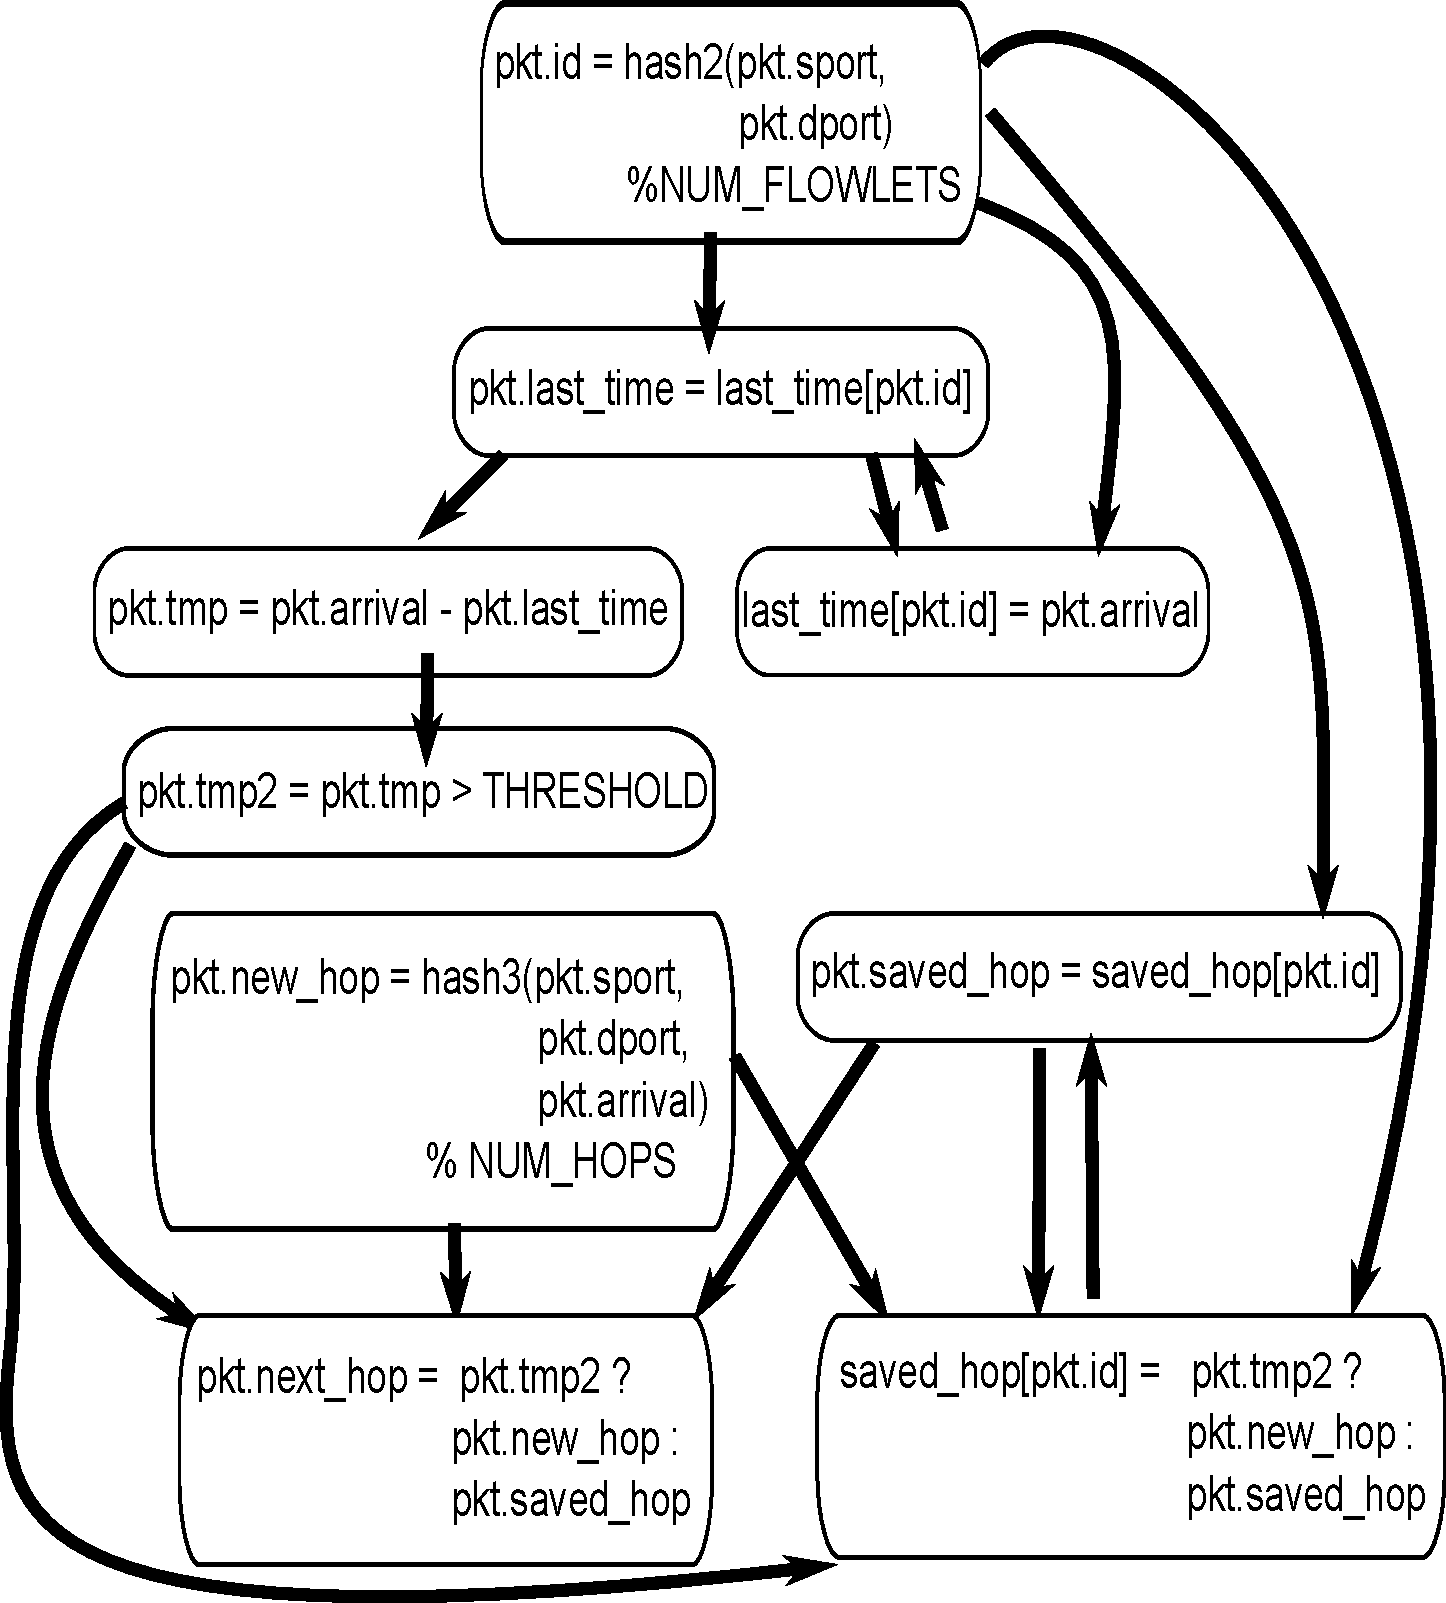
\includegraphics[width=\columnwidth]{deps.pdf}
  \caption{Dependency before condensing SCCs}
  \label{fig:partitioning_before}
\end{minipage}
%
\vrule\quad
%
\begin{minipage}{0.5\textwidth}
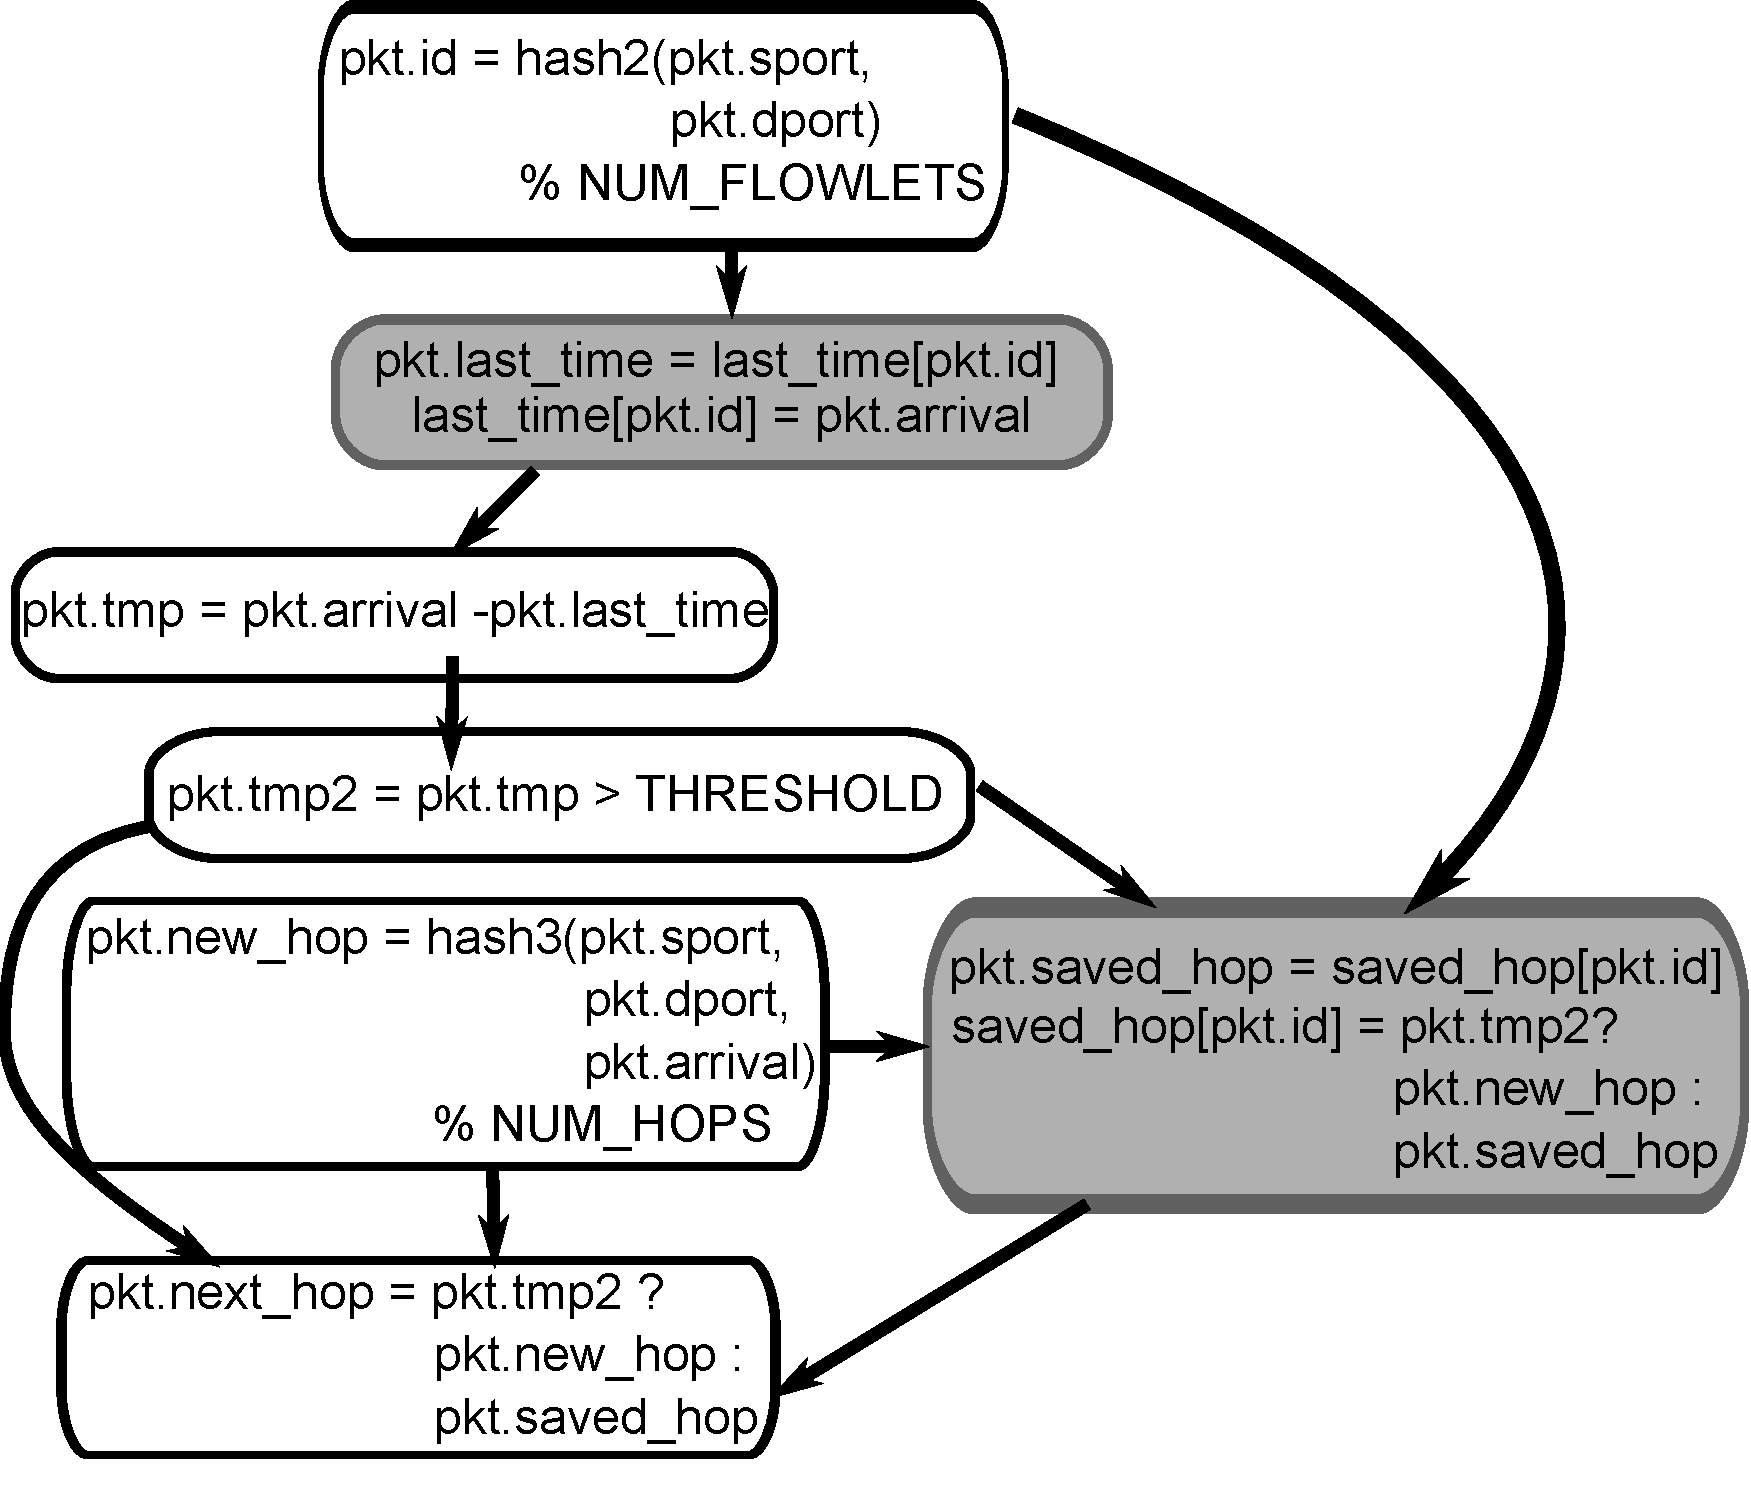
\includegraphics[width=\columnwidth]{scc.pdf}
\caption{Dependency graph after condensing SCCs}
\label{fig:partitioning_after}
\end{minipage}
\end{figure*}

\subsection{Code generation}
\label{ss:code_gen}
The final pass of the compiler determines if the code for the Pipelined Virtual
Switch Machine in the previous pass can be compiled to a hardware target (in
our case, a \absmachine machine). To do so, we consider three limits present in
any \absmachine machine: resource limits on the number of pipeline stages and
the width of each pipeline stage, and computational limits on atoms within a
stage.

\paragraph{Resource limits}
The problem of handling resource limits is an instance of resource-constrained
scheduling, where a dependence graph is scheduled subject to precedence and
resource constraints. This problem is NP-hard, and so we develop a simple
heuristic.  We scan each pipeline stage in the codelet pipeline starting from
the first to check if it violates the stage-width limit. If so, we move an
arbitrarily chosen codelet from that stage into the next one, creating a new
stage if required.  We continue until all stage-width limits are satisfied. We
now count the number of stages to check if it exceeds the limit on the number
of stages, and reject the code if so.

\paragraph{Computational limits}
Next, we determine if codelets in the pipeline map one-to-one to atoms provided
by the \absmachine machine. In general, codelets have multi-line bodies that
need to execute atomically. For instance, updating the state variable
\texttt{saved\_hop} in Figure~\ref{fig:flowlet_pipeline} requires a read
followed by a conditional write.  It is not apparent whether such codelets can
be mapped to an available atom. We develop a new technique to determine the
implementability of codelets, on a \absmachine machine that provide an atom
template.

First, each atom template is parameterized, where the parameters determine the
actual functionality provided by the atom.  For instance,
Figure~\ref{fig:alu_diag} shows a hardware circuit that is capable of
performing stateful addition or subtraction, depending on the value of the
constant and which output is selected from the multiplexer.  Its atom template
 is shown in Figure~\ref{fig:alu_in_sketch}, where {\tt choice}
and {\tt constant} represent the tunable parameters.  Each codelet can be
viewed as a functional specification of the atom.  With that in mind, the
mapping problem is equivalent to searching for the value of the parameters to
configure the atom such that it implements the provided specification.

While many algorithms can be used to perform the search, in the \pktlanguage
compiler we use the SKETCH program synthesizer~\cite{sketch_asplos} for this
purpose, as the atom templates can be easily expressed using SKETCH, while
SKETCH also provides efficient search algorithms and has been used for similar
purposes across different domains~\cite{bitstreaming, lifejoin, qbs, chlorophyll}.

As an illustration, assume we want to map the codelet {\tt x=x+1} to the atom
template shown in Figure~\ref{fig:alu_in_sketch}. The \pktlanguage compiler
feeds in the codelet and the atom template into SKETCH
(Figure~\ref{fig:sketch}), and SKETCH will search for possible values of the
parameters such that the resulting atom performs the same functionality as the
codelet, for all possible input values of {\tt x}.  In this case this is done
by setting {\tt choice=0} and {\tt constant=1}.  In contrast, if the codelet
{\tt x=x*x} was supplied as the specification, SKETCH will return an error as
no such parameter value exists. To minimize search time, the range of possible
inputs and parameter values need to be specified in the template (e.g., all 8
bit integers), and our experiments show that the search finishes quickly,
taking 10 secs at most.

%%\begin{figure}[!b]
%%  \begin{center}
%%  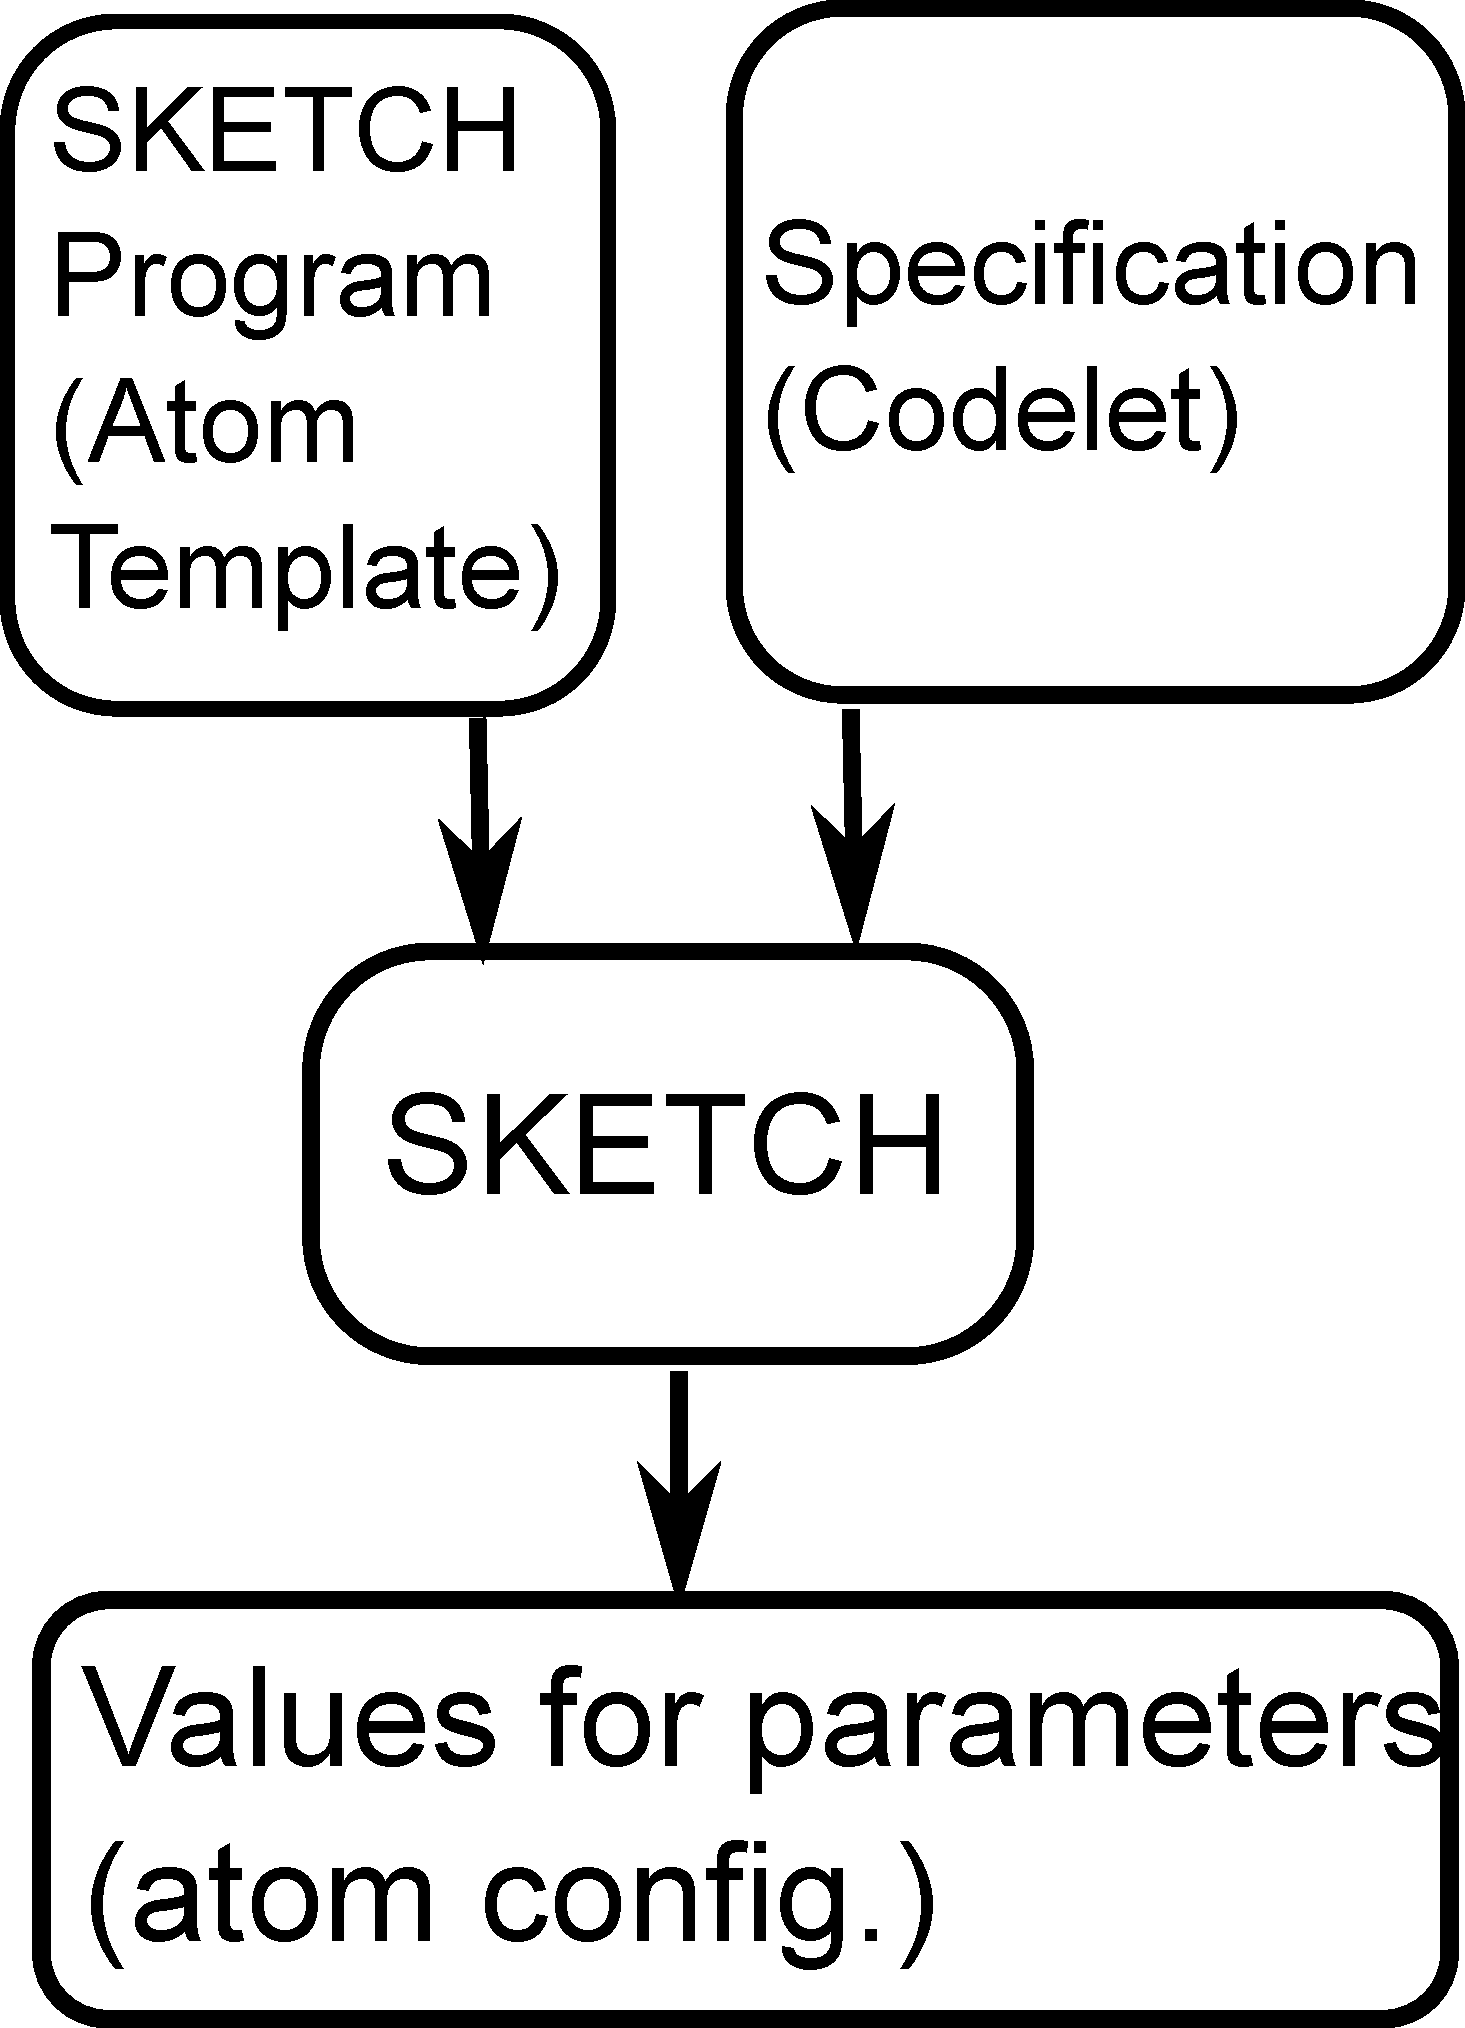
\includegraphics[width=0.4\columnwidth]{sketch.pdf}
%%  \caption{Overview of SKETCH and its application to atom configuration}
%%  \label{fig:sketch}
%%  \end{center}
%%\end{figure}

\begin{figure}[h]
  \begin{minipage}{0.4\columnwidth}
  \begin{center}
  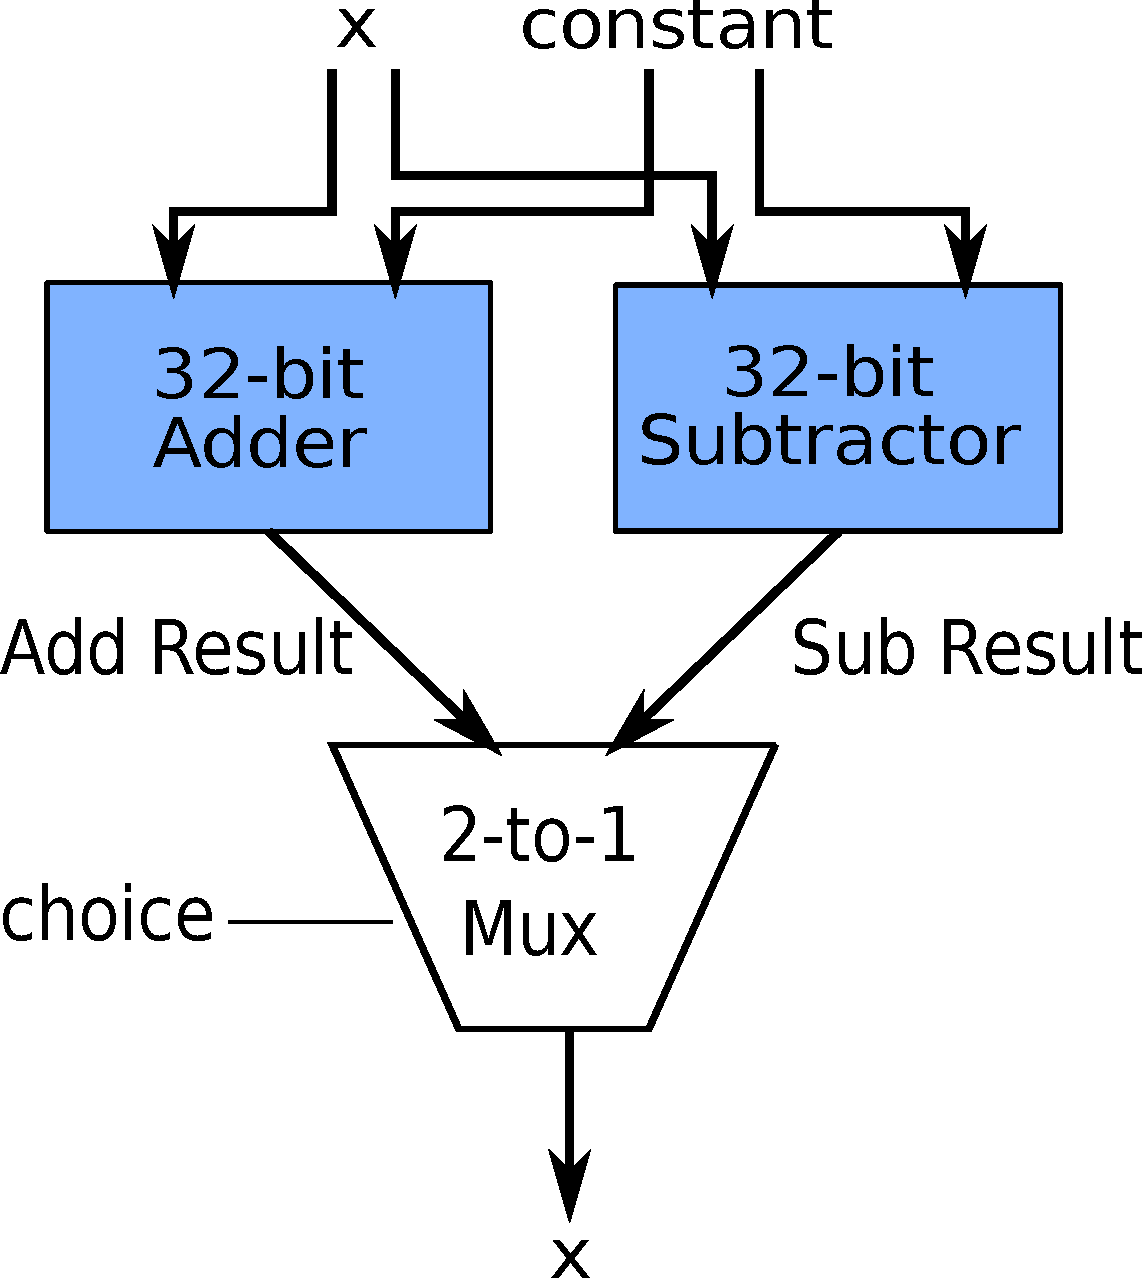
\includegraphics[width=\columnwidth]{circuit.pdf}
  \end{center}
  \caption{Circuit for an atom that can add or subtract a constant from a state variable.}
  \label{fig:alu_diag}
  \end{minipage}
  \hspace{0.05\columnwidth}
  \begin{minipage}{0.55\columnwidth}
  \begin{lstlisting}
  bit choice = ??;
  int constant = ??;
  if (choice) {
    x = x + constant;
  } else {
    x = x - constant;
  }
  \end{lstlisting}
  \caption{Circuit representation as an atom template.}
  %Each ``??(n)'' represents a hole that can be filled in with values in $[0, 2^n -1]$.}
  \label{fig:alu_in_sketch}
  \end{minipage}
\end{figure}

% TODO: Simplify this considerably.
% Also, per George, stress clearly what is new relative to standard compiler techniques.
\subsection{Discussion}
The \pktlanguage compiler borrows many techniques from the compiler literature.
The \absmachine architecture, however, poses unique challenges for compilation
requiring a synthesis of techniques that, to the best of our knowledge, is
novel. Further, as we illustrate throughout this section, constraining
\pktlanguage for deterministic performance simplifies the \pktlanguage
compiler relative to mainstream compilers for imperative languages.

This procedure is known as
if-conversion~\cite{if_conversion}. Unlike traditional languages, performing
if-conversion in \pktlanguage is easy as there is no unstructured control
flow.  
%%State variables are already in SSA: after their flanks
%%have been added, every state variable is written exactly once in the write
%%flank.  While general algorithms for computing the SSA are fairly
%%involved~\cite{ssa}, \pktlanguage's SSA computation is simpler because it runs
%%after if conversion and hence operates on straight-line code. 
